\documentclass{article}
\usepackage[utf8]{inputenc}
\usepackage{graphicx}
\graphicspath{ {./} }

% \title{EulerAlgoGCD}
% \author{Glaives De V�rit�}
% \date{December 2022}
\begin{document}
\begin{flushleft}

\textbf{Algorithm I} (\textit{Construct a proof}). Given a positive integer \textit{n}, this algorithm will output a proof that \textit{P}(\textit{n}) is true.
\vspace{4mm}
\par \textbf{I1.} [Prove \textit{P}(1).] Set $\textit{k}\gets1$, and, according to (a), output a proof of \textit{P}(1).
\vspace{2mm}
\par \textbf{I2.} [\textit{k} = \textit{n}?] If \textit{k} = \textit{n}, terminate the algorithm; the required proof has been output.
\vspace{2mm}
\par \textbf{I3.} [Prove \textit{P}(\textit{k}+ 1)] According to (b), output a proof that ``If all of \textit{P}(1), ..., \textit{P}(\textit{k}) are true, then \textit{P}(\textit{k} + 1) is true.'' Also output ``We have already proved \textit{P}(1), ..., \textit{P}(\textit{k}); hence \textit{P}(\textit{k} + 1) is true.''
\vspace{2mm}
\par \textbf{I4.} [Increase \textit{k}.] Increase \textit{k} by 1 and go to step I2.
\vspace{3mm}
\par 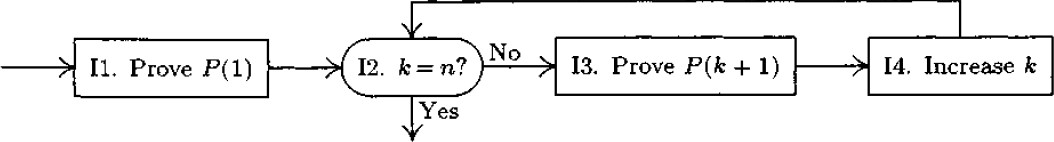
\includegraphics[width=\textwidth]{scheme}
\vspace{3mm}
\par \textbf{Remarks:}
\vspace{2mm}
\par a) Give a proof that \textit{P}(1) is true.
\vspace{2mm}
\par b) Give a proof that ``if all of \textit{P}(1), \textit{P}(2), ..., \textit{P}(\textit{n}) are true, then \textit{P}(\textit{n} + 1) is also true''; this proof should be valid for any positive integer \textit{n}.
\end{flushleft}
\end{document}

